\section{Supersafety to Perfect Timeliness}\label{sec:backward-reduction}

We now construct a perfectly timely protocol $\Pi^*$
using a black-box reduction from a supersafe, and live($u$) protocol $\Pi$.
Each honest party $P$, executing the $\Pi^*$ protocol, runs a
full node of protocol $\Pi$.
The main idea is that, since ledgers are supersafe, we can simply
ascribe to each new transaction the round at which it first appeared on our ledger.
% The ledger of party $P$ for protocol $\Pi$ and $\Pi^*$ is denoted as $\Ledger[][P][r]$ and
% $\Ledger[*][P][r]$ respectively.
% To construct temporal ledger $\Ledger[*][][r]$,
% new transactions appearing in
% $\Ledger[][][r]$ are appended to $\Ledger[*][][r - 1]$ with recorded round $r$.
This reduction is illustrated in Figure~\ref{fig:backward-reduction}
and Algorithm~\ref{alg:backward-reduction}.

\begin{figure}
  \centering
  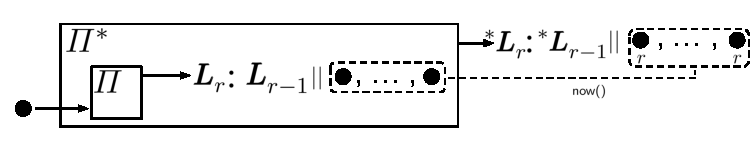
\includegraphics[width=0.9\columnwidth,keepaspectratio]{figures/backward-reduction.pdf}
  \caption{The reduction from Supersafety
    (the $\Pi$ protocol) to Perfect Timeliness (the $\Pi^*$ protocol).
    New transactions of $\Ledger[][][r]$ are included in
    $\Ledger[*][][r]$ with recorded round $r$.
  }
 \label{fig:backward-reduction}
\end{figure}

\import{./}{algorithms/algorithm-backward-reduction.tex}

%We now prove that protocol $\Pi^*$ is perfectly timely.

\begin{theorem}[Supersafety to Perfect Timeliness] \label{thm:backward-reduction}
  An execution of $\Pi^*$ is perfectly timely, supersafe, and live($u$), if the execution of
  $\Pi$ is supersafe and live($u$).
\end{theorem}
\begin{proof}
  Timeliness requirements (1) and (2) are directly satisfied.
  For (3) consider any honest party $P$ and any rounds $r_1 \leq r_2$.
  Only transactions with recorded round greater
  than $r_1$ appear in ledger $\Ledger[*][P][r_2]{[|\Ledger[*][P][r_1]|{:}]}$.
  Hence, $\Pi^*$ is timely with parameter $v = 0$.
  Supersafety and liveness($u$) follow from those of $\Pi$.
  \Qed
\end{proof}

\atnote{We define clients in the beginning, but we only use them here.}
When a late joining client if activated by the environment,
first, it obtains all past transactions from its $\Pi$ instance.
However, there is no way to calculate their recorded round.
To allow this, each node party is required to run an
additional instance of $\Pi$. We call this new instance $\Pi_2$,
and the existing one, which operates in the same way, $\Pi_1$.
Let $\Ledger[1]$ and $\Ledger[2]$ be the output ledgers
of $\Pi_1$ and $\Pi_2$ respectively.
The output ledger $\Ledger[*]$ of the nodes remains the same.
Instance $\Pi_2$ is used as follows:
In every round $r$, all honest nodes $P$ introduce a transaction
which contains ledger $\Ledger[*][P][r]$.
We parameterize $\Pi_2$ with the following transaction validity language:
Valid transactions contain any ledger $\hat \Ledger \preccurlyeq \Ledger[*][P][r]$.
The protocol is illustrated in Figure~\ref{fig:client-support}.

A late joining client, first synchronizes $\Pi_1$ and $\Pi_2$ with the rest
of the peers. Once synchronized, the recorded rounds of new
transactions appearing in $\Ledger[1]$ are continuously stored.
Due to safety, liveness and the validity rule of $\Pi_2$,
the client can read ledger $\Ledger[2]$ to find out the
recorded rounds of past transactions.
Eventually, all past transaction recorded rounds are included in $\Ledger[2]$
and the client can construct the correct temporal ledger $\Ledger[*]$.
At this point we say that the client is booted.

\begin{figure}
  \centering
  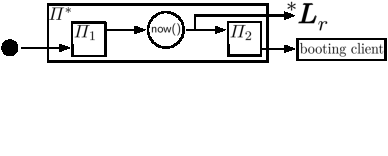
\includegraphics[width=0.7\columnwidth,keepaspectratio]{figures/clients.pdf}
  \caption{Client support for $\Pi$.
  }
 \label{fig:client-support}
\end{figure}